% !TeX root = ../Fundamental-Physics-B.tex
% 第 2.4 节：绳、滑轮与连接体模型

\section{绳、滑轮与连接体模型}

绳、滑轮和连接体问题的核心是：先明确理想模型条件，再根据约束关系把多个物体的加速度联系起来。若只凭直觉把张力写成 $mg$，或把所有物体的加速度都直接写成相等，往往会导致错误。

\subsection{理想轻绳与理想滑轮}

理想轻绳通常满足以下条件：
\begin{enumerate}
    \item 绳的质量忽略不计；
    \item 绳不可伸长；
    \item 张力方向沿绳；
    \item 同一根轻绳上的张力大小处处相等。
\end{enumerate}

若滑轮也可视为理想滑轮，即滑轮质量和轴摩擦均忽略，则滑轮只改变张力方向，不改变张力大小。因此通过理想定滑轮的同一根轻绳两侧张力大小相等。

\begin{attention}{张力不一定等于重力}{ch2:tension-not-mg}
绳的张力由动力学方程决定。只有物体静止或匀速直线运动且竖直方向只受重力和张力时，才有 $T=mg$。若物体有竖直加速度，一般应写
\[
    T-mg=ma
\]
或按所选正方向列式。
\end{attention}

\subsection{连接体问题中的整体法与隔离法}

连接体问题常用两种方法。

\textbf{整体法}：把多个物体看成一个系统。系统内力在整体方程中相互抵消，适合求系统共同加速度。

\textbf{隔离法}：把其中一个物体单独取出。隔离法适合求物体之间的接触力、绳中张力或某个接触面的摩擦力。

对于轻绳不可伸长的系统，应先写绳长约束，再对时间求导得到速度和加速度关系。最简单的定滑轮模型中，绳两端物体沿绳方向的加速度大小相等、方向相反；动滑轮问题中则不能机械套用“加速度相等”，必须从绳长不变条件出发。

\subsection{例题 2.5：定滑轮拉重物时人对地面的压力}

\begin{figure}[htbp]
    \centering
    \IfFileExists{images/ex-2-5-original.png}{%
        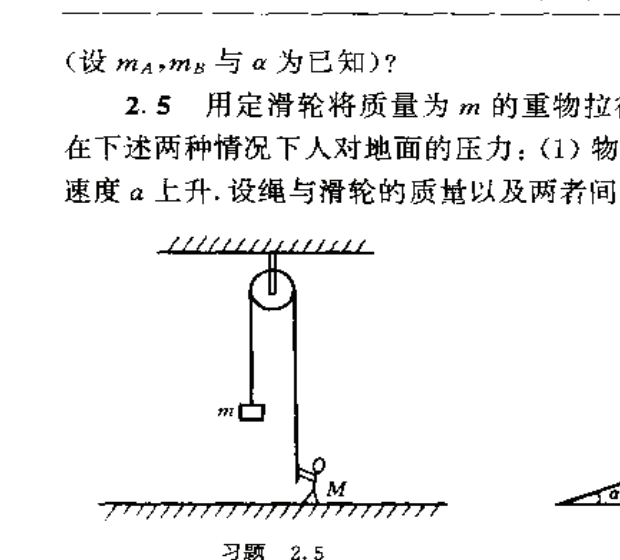
\includegraphics[width=0.62\textwidth]{images/ex-2-5-original.png}
    }{%
        \fbox{\parbox{0.62\textwidth}{\centering 原题图 2.5 预留位置：请将裁切后的图片命名为 \texttt{ex-2-5-original.png} 并放入 \texttt{images/} 目录。}}
    }
    \caption{习题 2.5 原题图}
\end{figure}

定滑轮和绳的质量、摩擦均忽略，因此绳中张力处处相等，记为 $T$。人受三个竖直方向的力：重力 $Mg$ 向下、地面对人的支持力 $N$ 向上、绳对人的拉力 $T$ 向上。人静止在地面上，故
\[
    N+T-Mg=0,
    \qquad
    N=Mg-T.
\]
人对地面的压力大小等于地面对人的支持力大小，即为 $N$。

\subsubsection*{（1）物体匀速上升}

物体匀速上升时加速度为零，对重物有
\[
    T-mg=0,
    \qquad
    T=mg.
\]
因此
\[
    \boxed{N=(M-m)g}.
\]

\subsubsection*{（2）物体以加速度 $a$ 上升}

取竖直向上为正方向。对重物有
\[
    T-mg=ma,
    \qquad
    T=m(g+a).
\]
所以人对地面的压力为
\[
    \boxed{N=Mg-m(g+a)=(M-m)g-ma}.
\]
若该表达式小于等于零，说明人将离开地面，地面对人的支持力不能再按静止接触条件求解。

\begin{center}
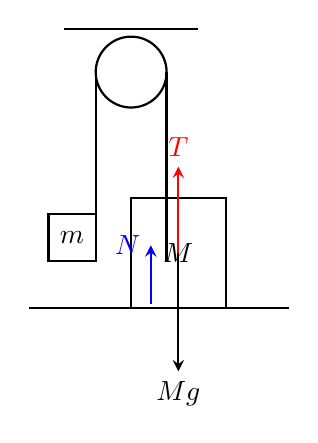
\begin{tikzpicture}[scale=1.0,>=stealth]
    \draw[thick] (0,3.0) circle (0.45);
    \draw[thick] (-0.45,3.0) -- (-0.45,1.2);
    \draw[thick] (0.45,3.0) -- (0.45,0.6);
    \draw[thick] (-0.85,3.55) -- (0.85,3.55);
    \draw[thick] (-0.45,1.2) rectangle (-1.05,0.6);
    \node at (-0.75,0.9) {$m$};
    \draw[thick] (0.0,0) -- (1.2,0) -- (1.2,1.4) -- (0.0,1.4) -- cycle;
    \node at (0.6,0.7) {$M$};
    \draw[thick] (-1.3,0) -- (2.0,0);
    \draw[->,thick,red] (0.6,0.7) -- (0.6,1.8) node[above] {$T$};
    \draw[->,thick] (0.6,0.7) -- (0.6,-0.8) node[below] {$Mg$};
    \draw[->,thick,blue] (0.25,0.05) -- (0.25,0.8) node[left] {$N$};
\end{tikzpicture}
\end{center}

\subsection{公式小结}

\begin{knowledge}{常用关系式}{ch2:newton-formula-summary}
\[
\begin{aligned}
&\text{牛顿第二定律：} && \sum \boldsymbol F=m\boldsymbol a,\\
&\text{动量形式：} && \sum \boldsymbol F=\dfrac{\mathrm d\boldsymbol p}{\mathrm dt},\\
&\text{重力：} && G=mg,\\
&\text{胡克定律：} && F=k|\Delta l|,\\
&\text{最大静摩擦力：} && f_{s,\max}=\mu_sN,\\
&\text{滑动摩擦力：} && f_k=\mu_kN,\\
&\text{理想轻绳定滑轮：} && T_1=T_2=T.
\end{aligned}
\]
使用这些公式前，必须先确认研究对象、参考系、接触关系和运动状态。
\end{knowledge}
